% !TeX spellcheck = es_ES
%%%%%%%%%%%%%%%%%%%%%%%%%%%%%%%%%%%%%%%%%
% Stylish Article
% LaTeX Template
% Version 2.1 (1/10/15)
%
% This template has been downloaded from:
% http://www.LaTeXTemplates.com
%
% Original author:
% Mathias Legrand (legrand.mathias@gmail.com) 
% With extensive modifications by:
% Vel (vel@latextemplates.com)
% Final ACS by:
% Juan Barbosa
% License:
% CC BY-NC-SA 3.0 (http://creativecommons.org/licenses/by-nc-sa/3.0/)
%
%%%%%%%%%%%%%%%%%%%%%%%%%%%%%%%%%%%%%%%%%
\documentclass[fleqn,11pt]{SelfArx}
%\usepackage[superscript]{cite}
\usepackage{wrapfig}
\usepackage{rotating}
\usepackage{subcaption}
\usepackage[numbers]{natbib}
%----------------------------------------------------------------------------------------
%	ARTICLE INFORMATION
%----------------------------------------------------------------------------------------

\JournalInfo{Fisicoqu\'imica avanzada, No. 1, 16/11/2018} % Journal information
\Archive{ }

\PaperTitle{Espectroscop\'ia de impedancias} %
%\Keywords{Keyword1 --- Keyword2 --- Keyword3} % Keywords - if you don't want any simply remove all the text between the curly brackets
%\newcommand{\keywordname}{Keywords} % Defines the keywords heading name

%----------------------------------------------------------------------------------------
%	ABSTRACT
%----------------------------------------------------------------------------------------

\Abstract{
}

%----------------------------------------------------------------------------------------

\begin{document}
	\flushbottom % Makes all text pages the same height
	
	\maketitle % Print the title and abstract box
	
	%\tableofcontents % Print the contents section
	
	\thispagestyle{empty} % Removes page numbering from the first page
	\renewcommand{\tablename}{Tabla} 
	
	
	%----------------------------------------------------------------------------------------
	%	ARTICLE CONTENTS
	%----------------------------------------------------------------------------------------
	
	\section*{Introducci\'on}
	La impedancia representa la oposici\'on que un circuito exhibe al flujo de una corriente sinusoidal.	
	
	the capacitor is a short circuit. Figure 9.15 illustrates this.
	As a complex quantity, the impedance may be expressed in rectan-
	gular form as
	Open circuit at
	high frequencies
	(a)
	where R = Re Z is the resistance and X = Im Z is the reactance. The
	reactance X may be positive or negative. We say that the impedance is
	inductive when X is positive or capacitive when X is negative. Thus,
	impedance Z = R + j X is said to be inductive or lagging since current
	lags voltage, while impedance Z = R - j X is capacitive or leading
	because current leads voltage. The impedance, resistance, and reactance
	are all measured in ohms. The impedance may also be expressed in polar
	form as
	
	En la última década, la Espectroscopía de Impedancia Electroquímica (EIS) se ha establecido como una de las herramientas analíticas más populares en la investigación de materiales. La técnica se está aplicando de manera amplia y efectiva a un gran número de áreas importantes de investigación y análisis de materiales, tales como estudios de corrosión; monitoreo de propiedades de polímeros, coloides y revestimientos electrónicos e iónicos; mediciones en almacenamiento de energía, baterías y sistemas relacionados con pilas de combustible; análisis biológicos y sensores biomédicos; mediciones en semiconductores y electrolitos sólidos. La EIS permite estudiar procesos como la adsorción, el transporte de carga y masa y la cinética de reacciones secuenciales y paralelas acopladas \cite{lvovich2012impedance}.
	
	Los datos de impedancia obtenidos experimentalmente para un sistema de electrodo/material pueden analizarse utilizando un modelo matemático exacto basado en una teoría física plausible que predice la impedancia teórica $Z_t(\omega)$ o mediante un circuito equivalente relativamente empírico, estimando los parámetros, cuyas predicciones de impedancia se pueden denotar con $Z_{ec}(\omega)$. Las desventajas de la EIS se asocian principalmente con posibles ambigüedades en la interpretación. Una complicación importante de los análisis basados en un circuito equivalente es que los elementos de circuito ideal representan propiedades constantes ideales. En estas condiciones, los elementos ideales del circuito pueden ser inadecuados para describir la respuesta eléctrica. Muchos han observado en el campo que el uso de elementos de impedancia distribuida (por ejemplo, los elementos de fase constante (CPE)) en el circuito equivalente ayudan en gran medida al proceso de ajuste de los datos de impedancia observada para una celda con propiedades distribuidas \cite{macdonald2005impedance}.

	El presente informe contiene los espectros de impedancia junto con los circuitos ajustados de disoluciones a diferentes concentraciones del electrolito y variando de los iones presentes.
	
	
	\section{Secci\'on experimental}
	Los espectros de impedancia fueron realizados en un sistema de tres electrodos: un electrodo de oro, un electrodo de Ag/AgCl y una barra de platino como electrodo de trabajo, de referencia y contraelectrodo respectivamente. El electrodo de trabajo de oro fue pulido con al\'umina (\ce{Al2O3}) de 1,00, 0,30 y 0,05 $\mu$m de diámetro sobre una almohadilla apropiada y posteriormente activado con voltamperometría cíclica (VC) usando 20 barridos desde -0,2 V hasta 1,6 V en agua. 
	
	Una solución 1,0 M de perclorato de litio fue preparada disolviendo 5,319 g de \ce{LiClO4} en 50 mL de agua, de esta solución se tomaron 12,5 mL los cuales fueron dispuestos en un balón aforado de 25 mL para obtener una solución 0,5 M. De manera análoga se obtuvo una solución 0,1 M usando 2,5 mL de la solución 1,0 M en 25 mL de agua. Una cuarta solución 0,1 M fue preparada disolviendo 0.266 g de \ce{LiClO4} en 25 mL de acetonitrilo, el cual fue previamente secado usando tamiz molecular. Finalmente, fue preparada una solución de sulfato de sodio 0,1 M usando 0,355 g de \ce{Na2SO4} los cuales fueron disueltos en un balón aforado de 25 mL. Cada activación del electrodo y cada medida de espectro de impedancia fue realizada después de gasificar la solución con nitrógeno durante 10 minutos.
	
	\begin{figure*}[h]
		\centering
		\begin{subfigure}[t]{0.49\textwidth}
			\centering
			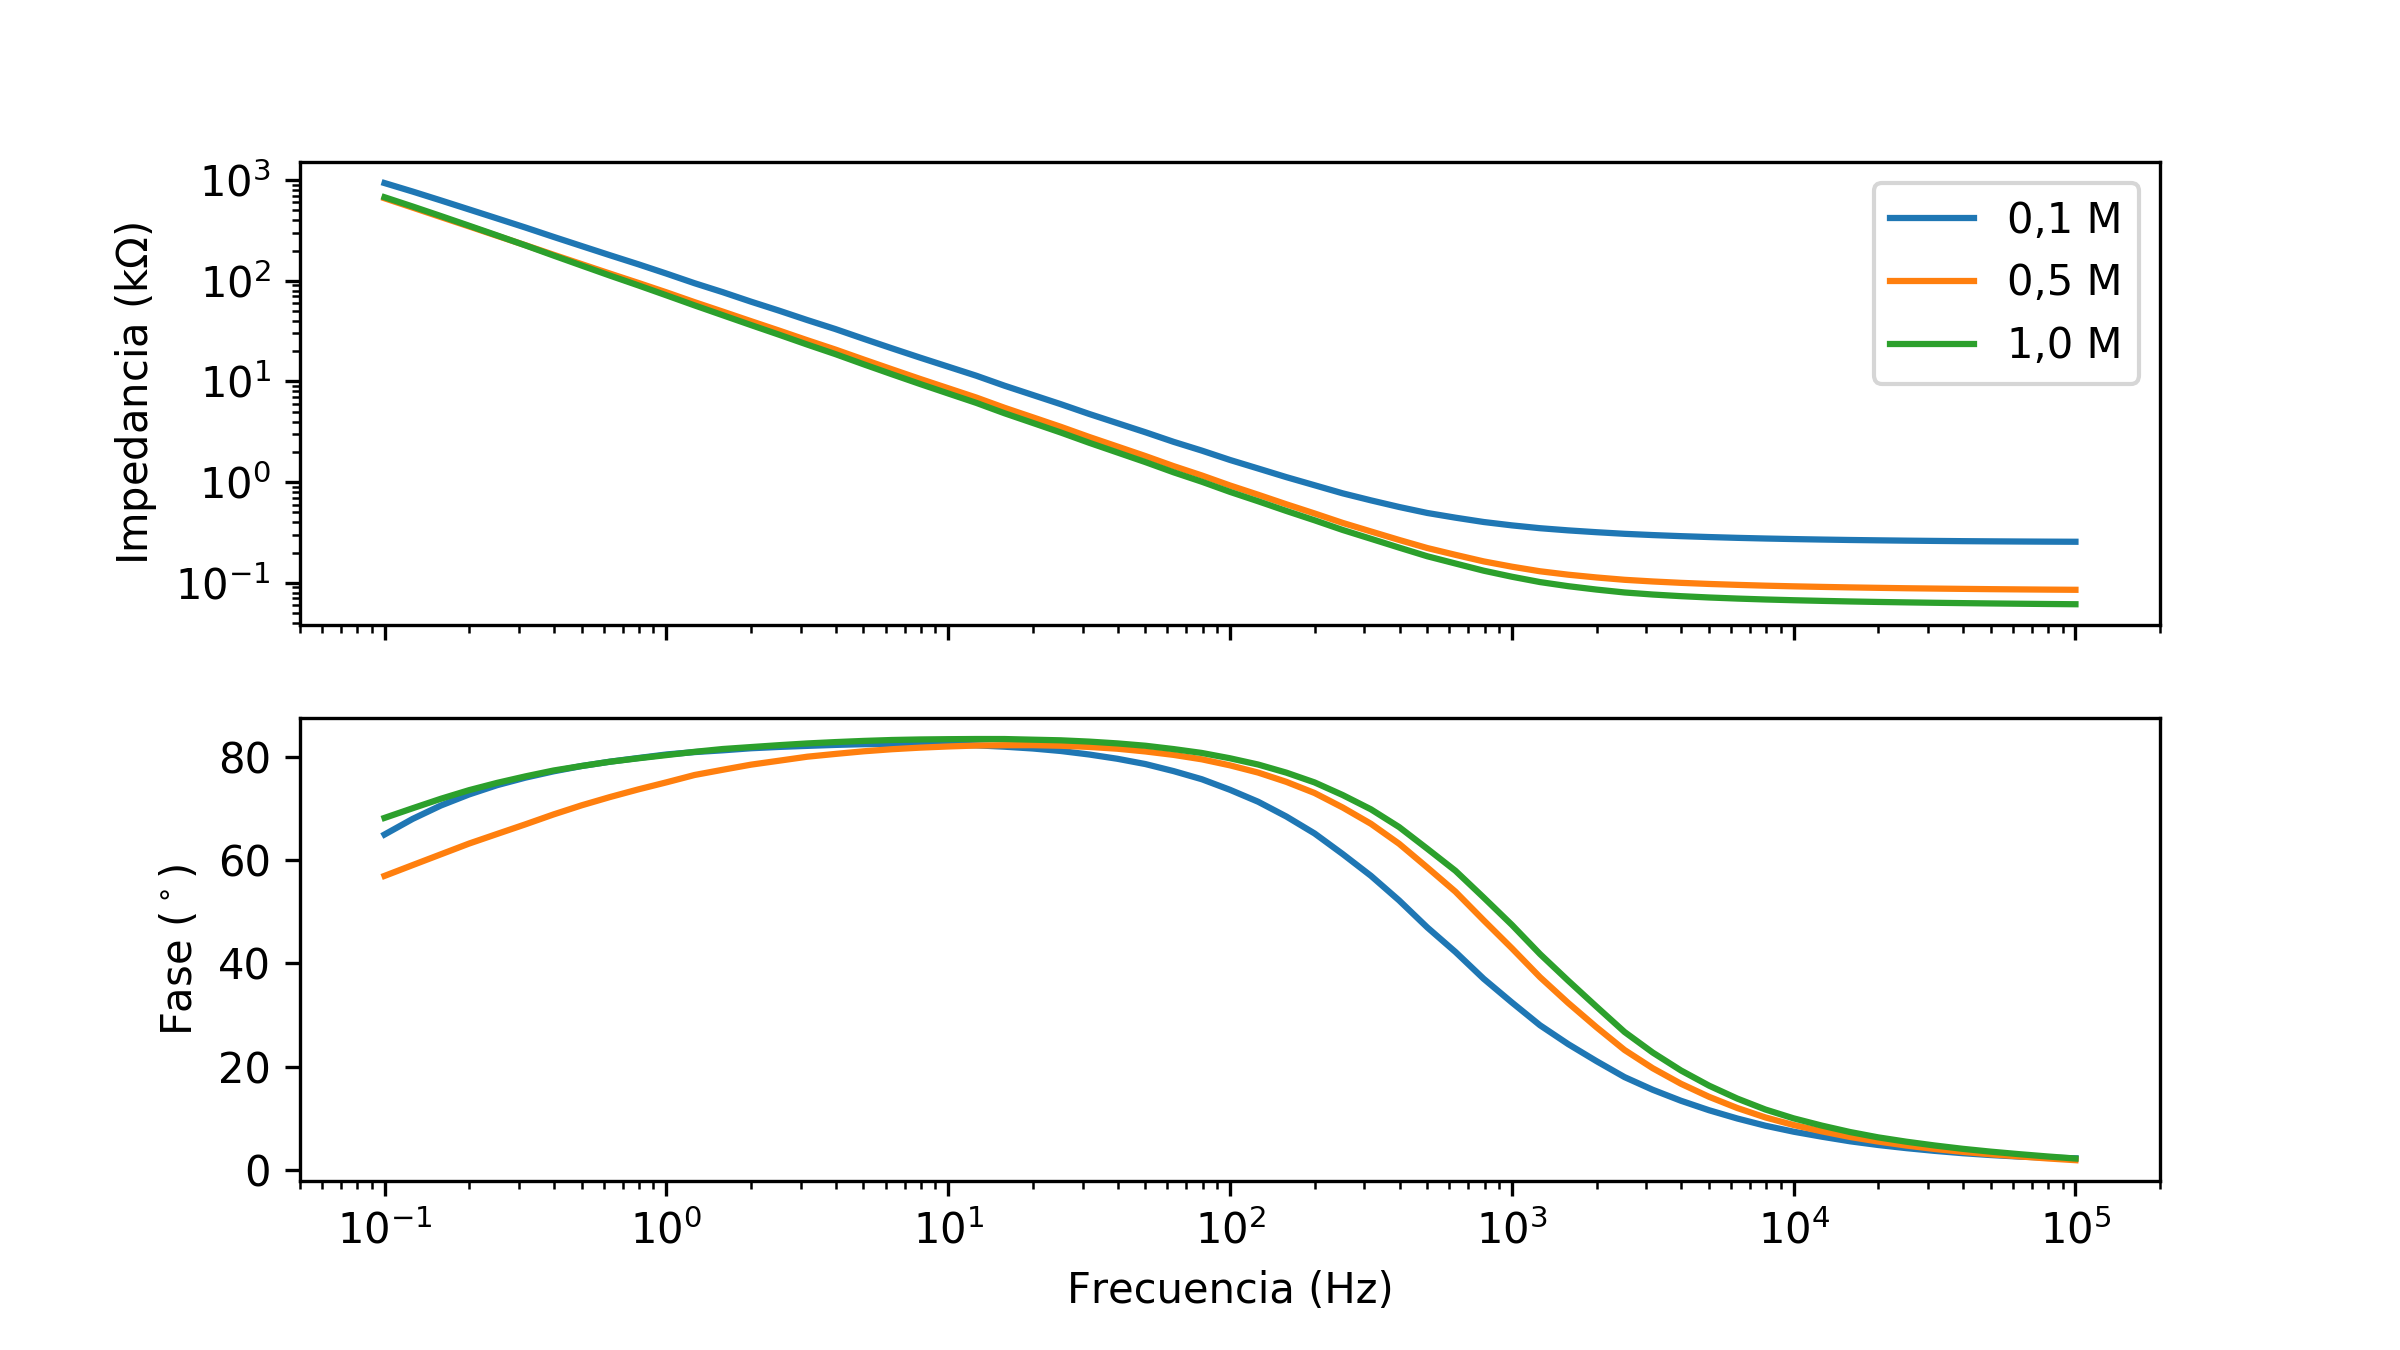
\includegraphics[width = \linewidth]{LiClO4_0,0V}
			\caption{0,0 V}
		\end{subfigure}
		\begin{subfigure}[t]{0.49\textwidth}
			\centering
			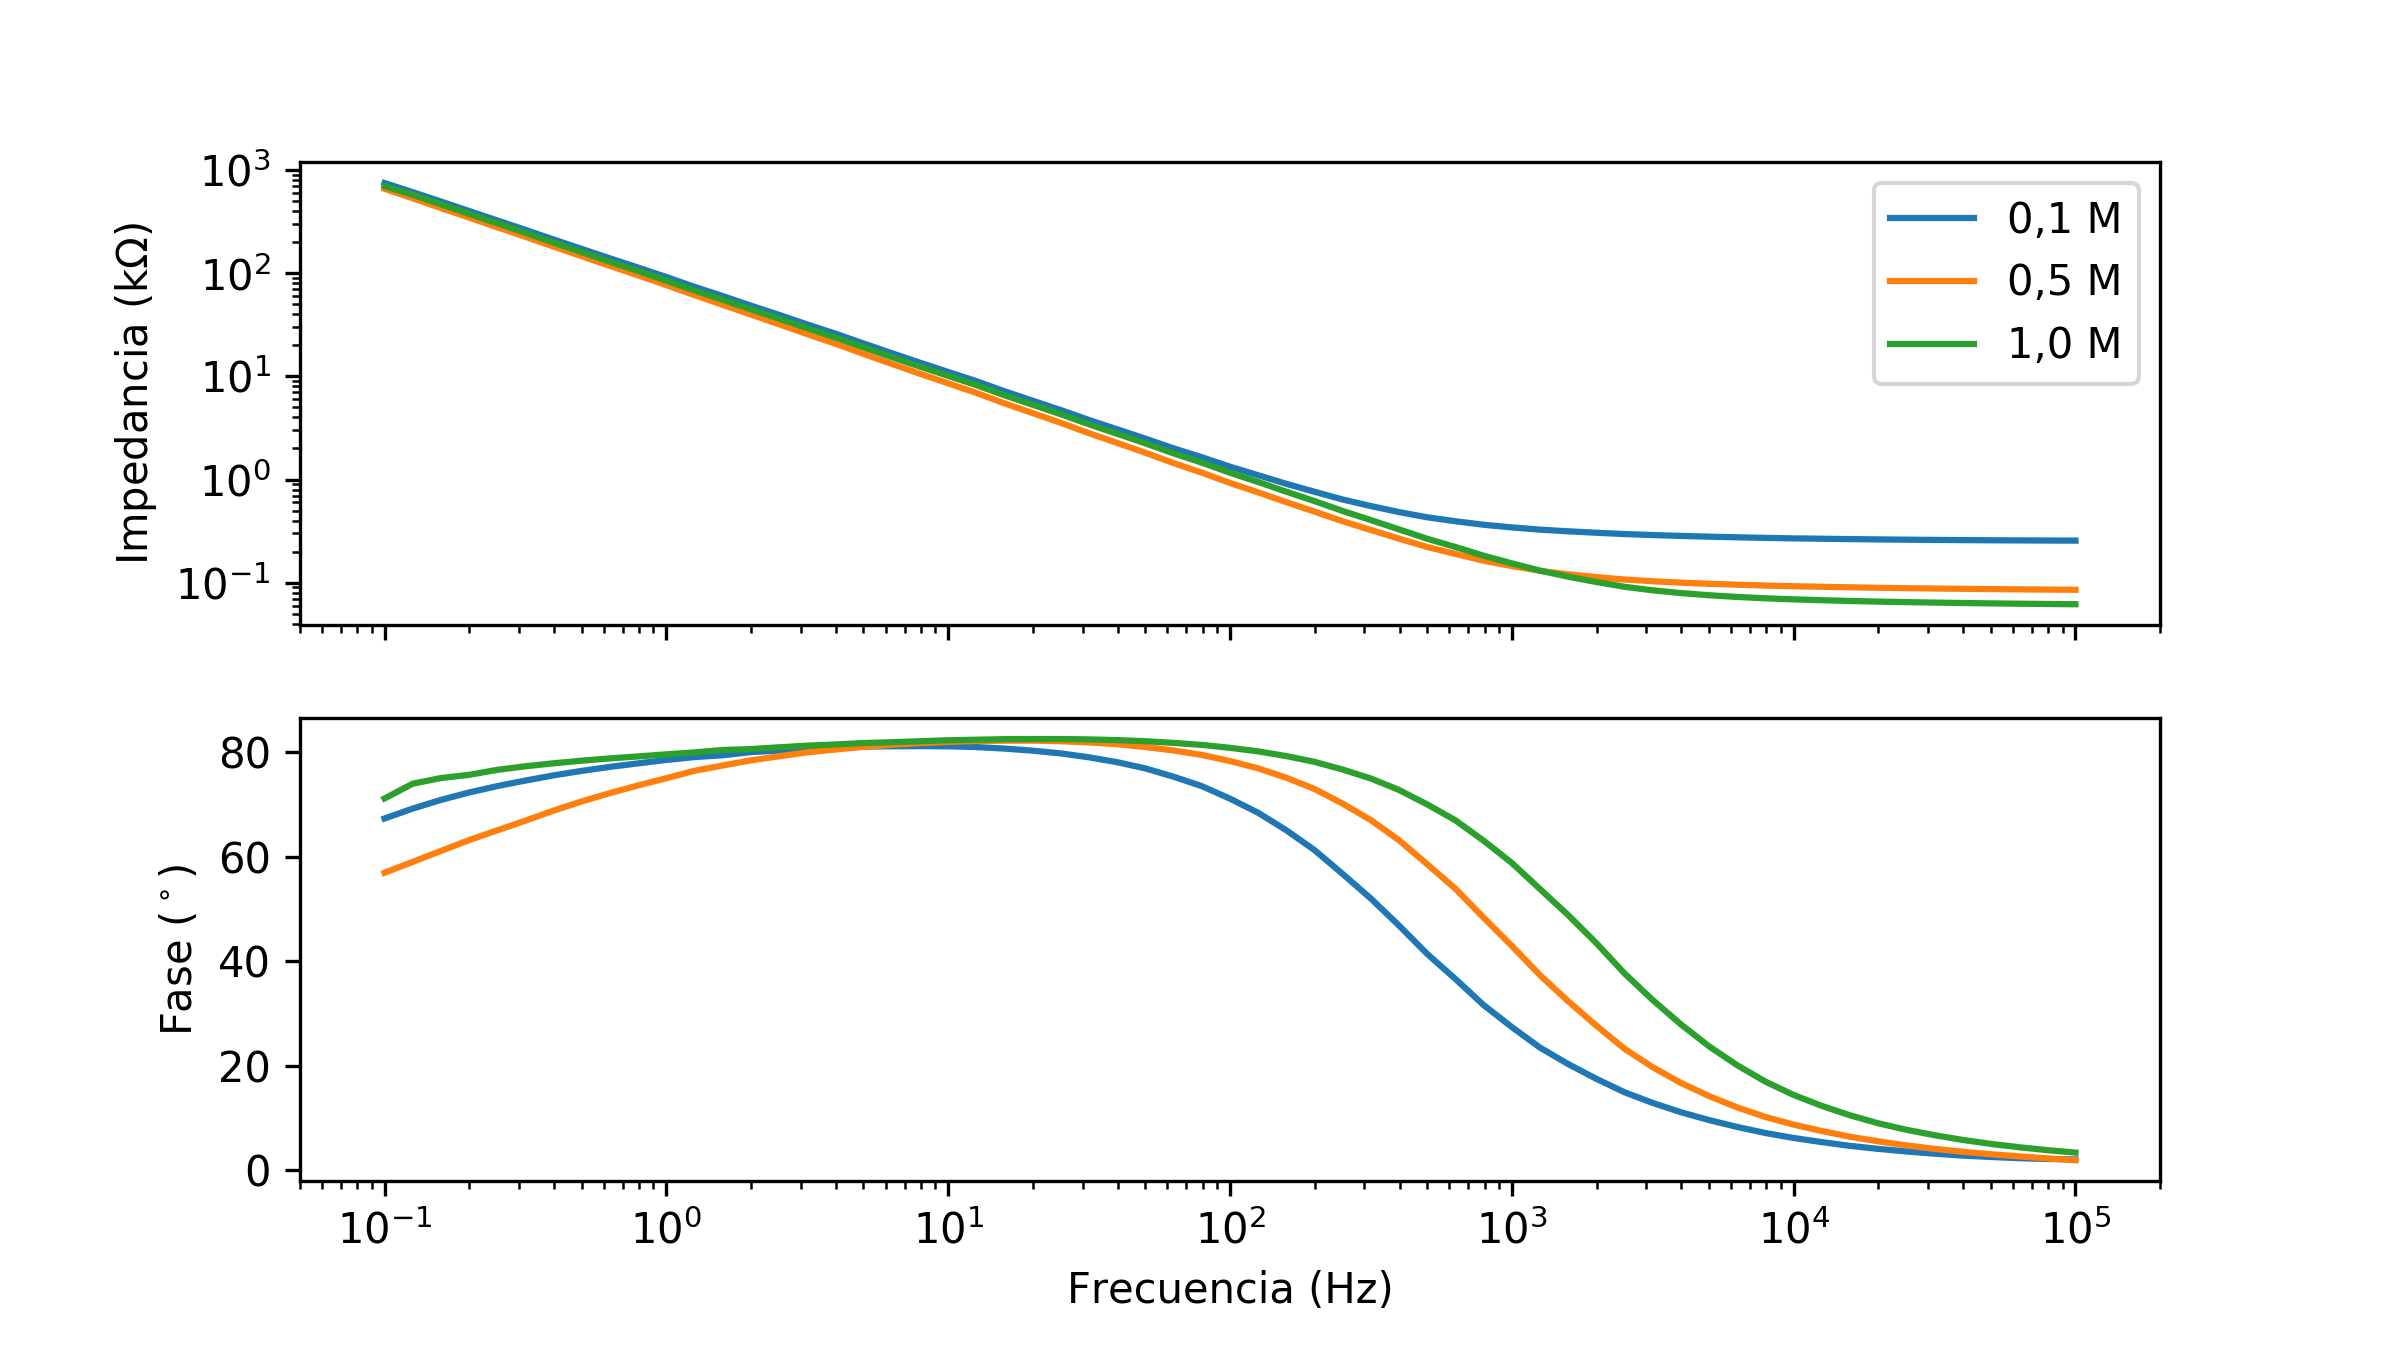
\includegraphics[width = \linewidth]{LiClO4_0,3V}
			\caption{0,3 V}
		\end{subfigure}
		\caption{Valores de impedancia en funci\'on de la frecuencia (superior) y diagrama de Bode (inferior) de la soluci\'on de \ce{LiClO4} a diferentes concentraciones.}
		\label{fig: concentraciones}
	\end{figure*}
	
	\section{Resultados y Discusi\'on}
	Como protocolo en las medidas electroquímicas, se tiene que limpiar cada electrodo apropiadamente. El electrodo de platino se somete a fuego de gas propano durante algunos segundos para que cualquier sustancia orgánica e inorgánica sea quemada. El electrodo de oro se pule con polvo de alúmina en agua para retirar cualquier partícula de la superficie yendo de particular de mayor tamaño a menor tamaño, sometiéndolo a ultrasonido entre cada cambio de tamaño de partícula. Posteriormente se hacen 20 barridos en VC para activar el electrodo, es decir, retirar cualquier partícula de alúmina que pudo quedar en la superficie. La superficie también se reorganiza en los barridos desde -0,20 V hasta 1,60 V respecto a Ag/AgCl. En la \autoref{fig: VC} se observa un pico de reducción entre 0,79 V y 0,8 V. Este pico fue aumentando tras cada barrido hasta que permaneció constante, esto se debe a la aparición de unos picos de oxidación entre 1,00 V y 1,25 V que fueron apareciendo mientras transcurrieron los barridos asociados a la formación de óxidos de oro superficial. También se observa una zona donde no hay corrientes faradaicas entre -0,20 V y 0,5 V, característico del oro, esto muestra que solo hay efecto de la doble capa eléctrica. Se estableció que el potencial de trabajo para la espectroscopía de impedancia electroquímica será 0,0 V y a 0,3 V ya que se garantiza que no hay reacciones a este potencial.
	\begin{figure}[h]
		\centering
		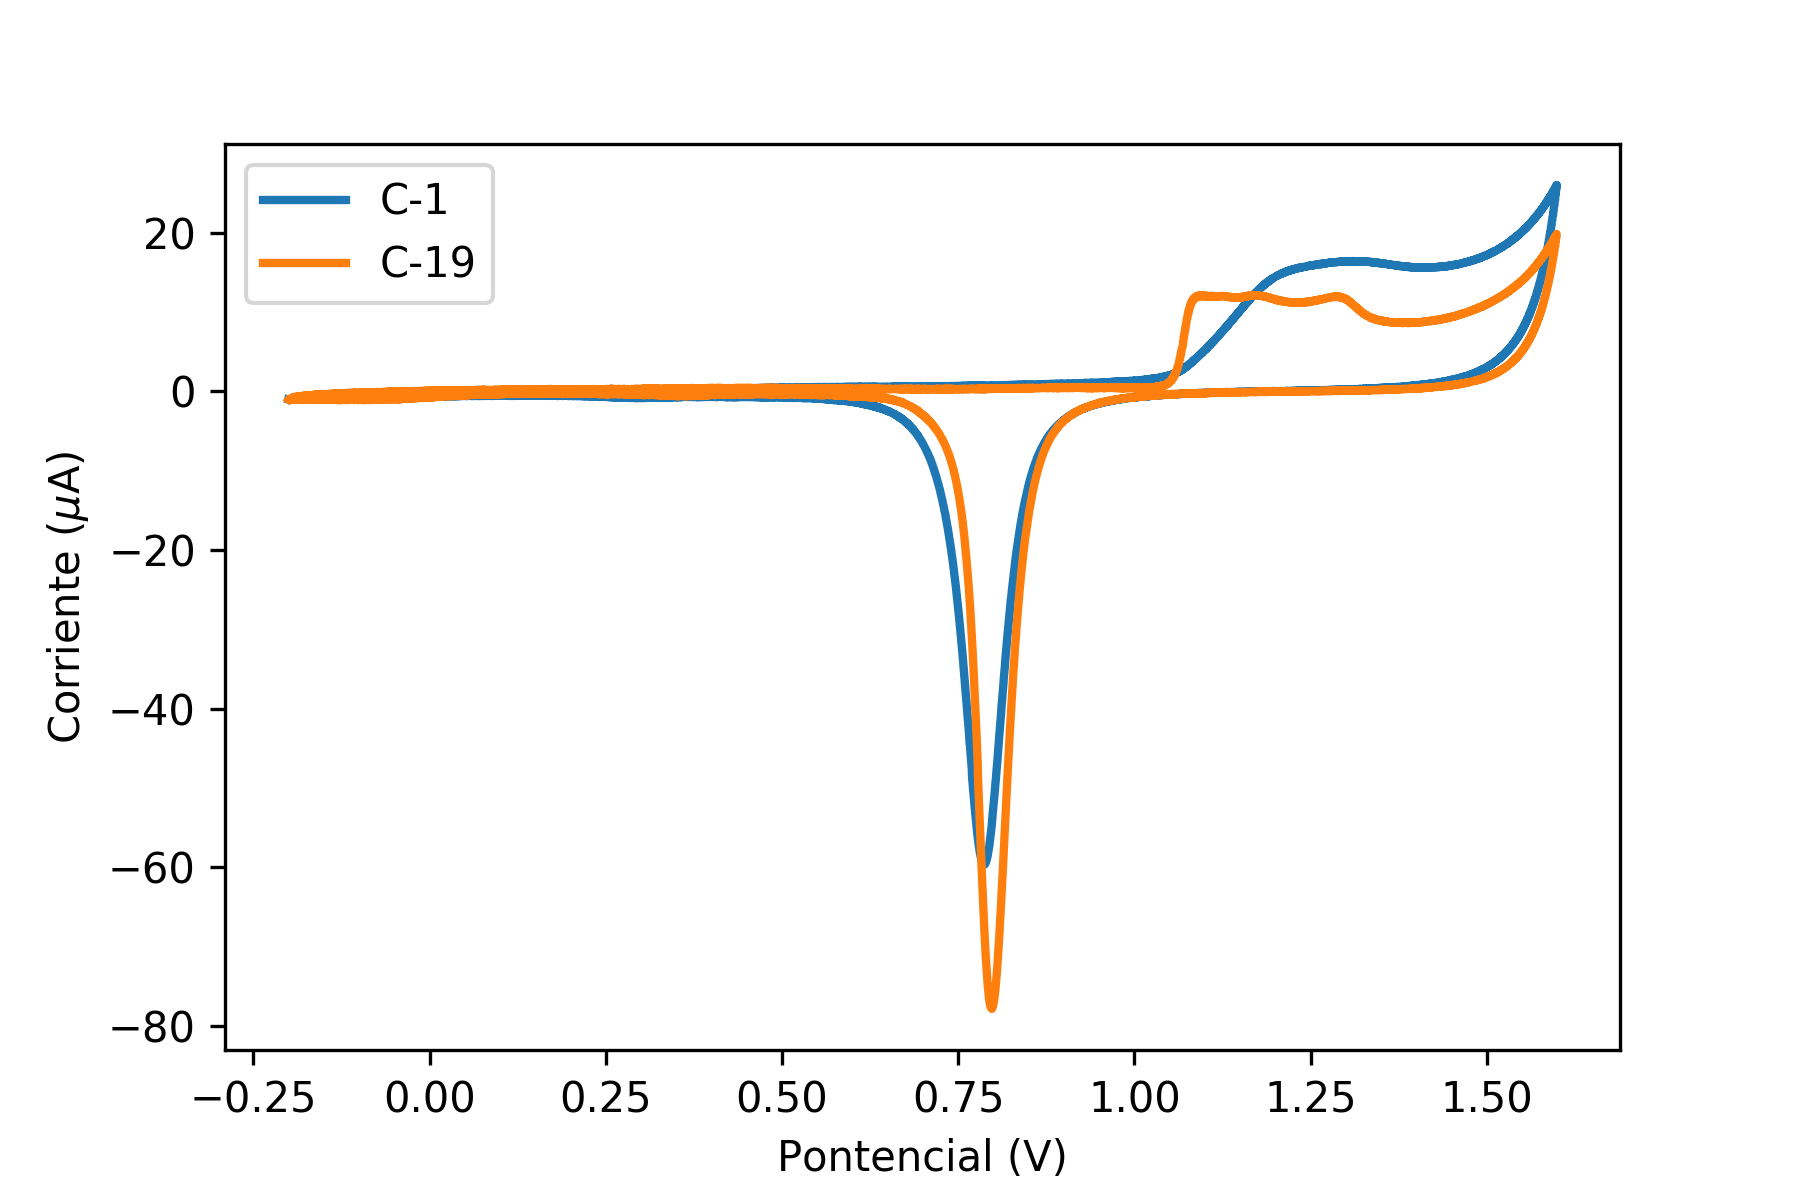
\includegraphics[width=\linewidth]{voltametrias}
		\caption{Voltametr\'ia c\'iclica de activaci\'on del electrodo de oro. Se muestra el primer y el d\'ecimo noveno barrido.}
		\label{fig: VC}
	\end{figure}

	\begin{table}[h]
		\caption{Valores de los elementos del circuito ajustado a los EIS a 0,0 V}
		\begin{tabular}{r|ll|ll}
			& \multicolumn{2}{c}{\textbf{0,1 M}} & \multicolumn{2}{c}{\textbf{1,0 M}} \\
			& \multicolumn{1}{c}{\textbf{Valor}} & \multicolumn{1}{c}{\textbf{\% Error}} & \multicolumn{1}{c}{\textbf{Valor}} & \multicolumn{1}{c}{\textbf{\% Error}} \\
			\hline
			R1 ($\Omega$) & 256 & 10,9 & 61,3 & 1,07 \\
			R2 (M$\Omega$) & 2.90 & 22,3 & 1,61 & 28,7 \\
			CPE ($\mu$F) & 1,60 & 1,66 & 2,3 & 3,7 \\
			n & 0,92 & 0,35 & 0,97 & 0,5 \\
			\hline
		\end{tabular}
		\label{tb: 0,0}
	\end{table}
	
	\begin{table}[h]
		\caption{Valores de los elementos del circuito ajustado a los EIS a 0,3 V}
		\begin{tabular}{r|ll|ll}
			& \multicolumn{2}{c}{\textbf{0,1 M}} & \multicolumn{2}{c}{\textbf{1,0 M}} \\
			& \multicolumn{1}{c}{\textbf{Valor}} & \multicolumn{1}{c}{\textbf{\% Error}} & \multicolumn{1}{c}{\textbf{Valor}} & \multicolumn{1}{c}{\textbf{\% Error}} \\
			\hline
			R1 ($\Omega$) & 257 & 0,71 & 61,9 & 0,53 \\
			R2 (M$\Omega$) & 2.67 & 16,0 & 2,73 & 23,3 \\
			CPE ($\mu$F) & 2,06 & 0,53 & 2,12 & 1,16 \\
			n & 0,92 & 0,12 & 0,93 & 0,24 \\
			\hline
		\end{tabular}
		\label{tb: 0,3}
	\end{table}
	
	En la \autoref{fig: concentraciones} se observa el cambio en las impedancias con respecto a la concentración. En primer lugar, se observa que la solución de menor concentración tiene más impedancia a mayores frecuencias (aquí es la parte de la ecuación que hablamos en la tarde), esto corresponde a que su resistencia entre el electrodo de referencia y la interfaz electrodo de trabajo-electrolito es mayor debido a la menor concentración de electrolito \cite{suarez2011} como transportador de carga. Esto lo corrobora los valores de R1 en la \autoref{tb: 0,0} y \autoref{tb: 0,3} que son mayores cuando la concentración es menor.  La \autoref{tb: 0,0} y \autoref{tb: 0,3} también muestra diferencias en el valor del elemento de fase constante CPE. Este elemento en el circuito llega a simular un condensador cuando el valor n es cercano a 1. Podemos observar que a mayor concentración hay un mayor valor en este elemento, esto significa que hay un mayor efecto en la doble capa eléctrica debido a la mayor presencia de iones en la superficie del electrolito. 
	
	\begin{figure}[h]
		\centering
		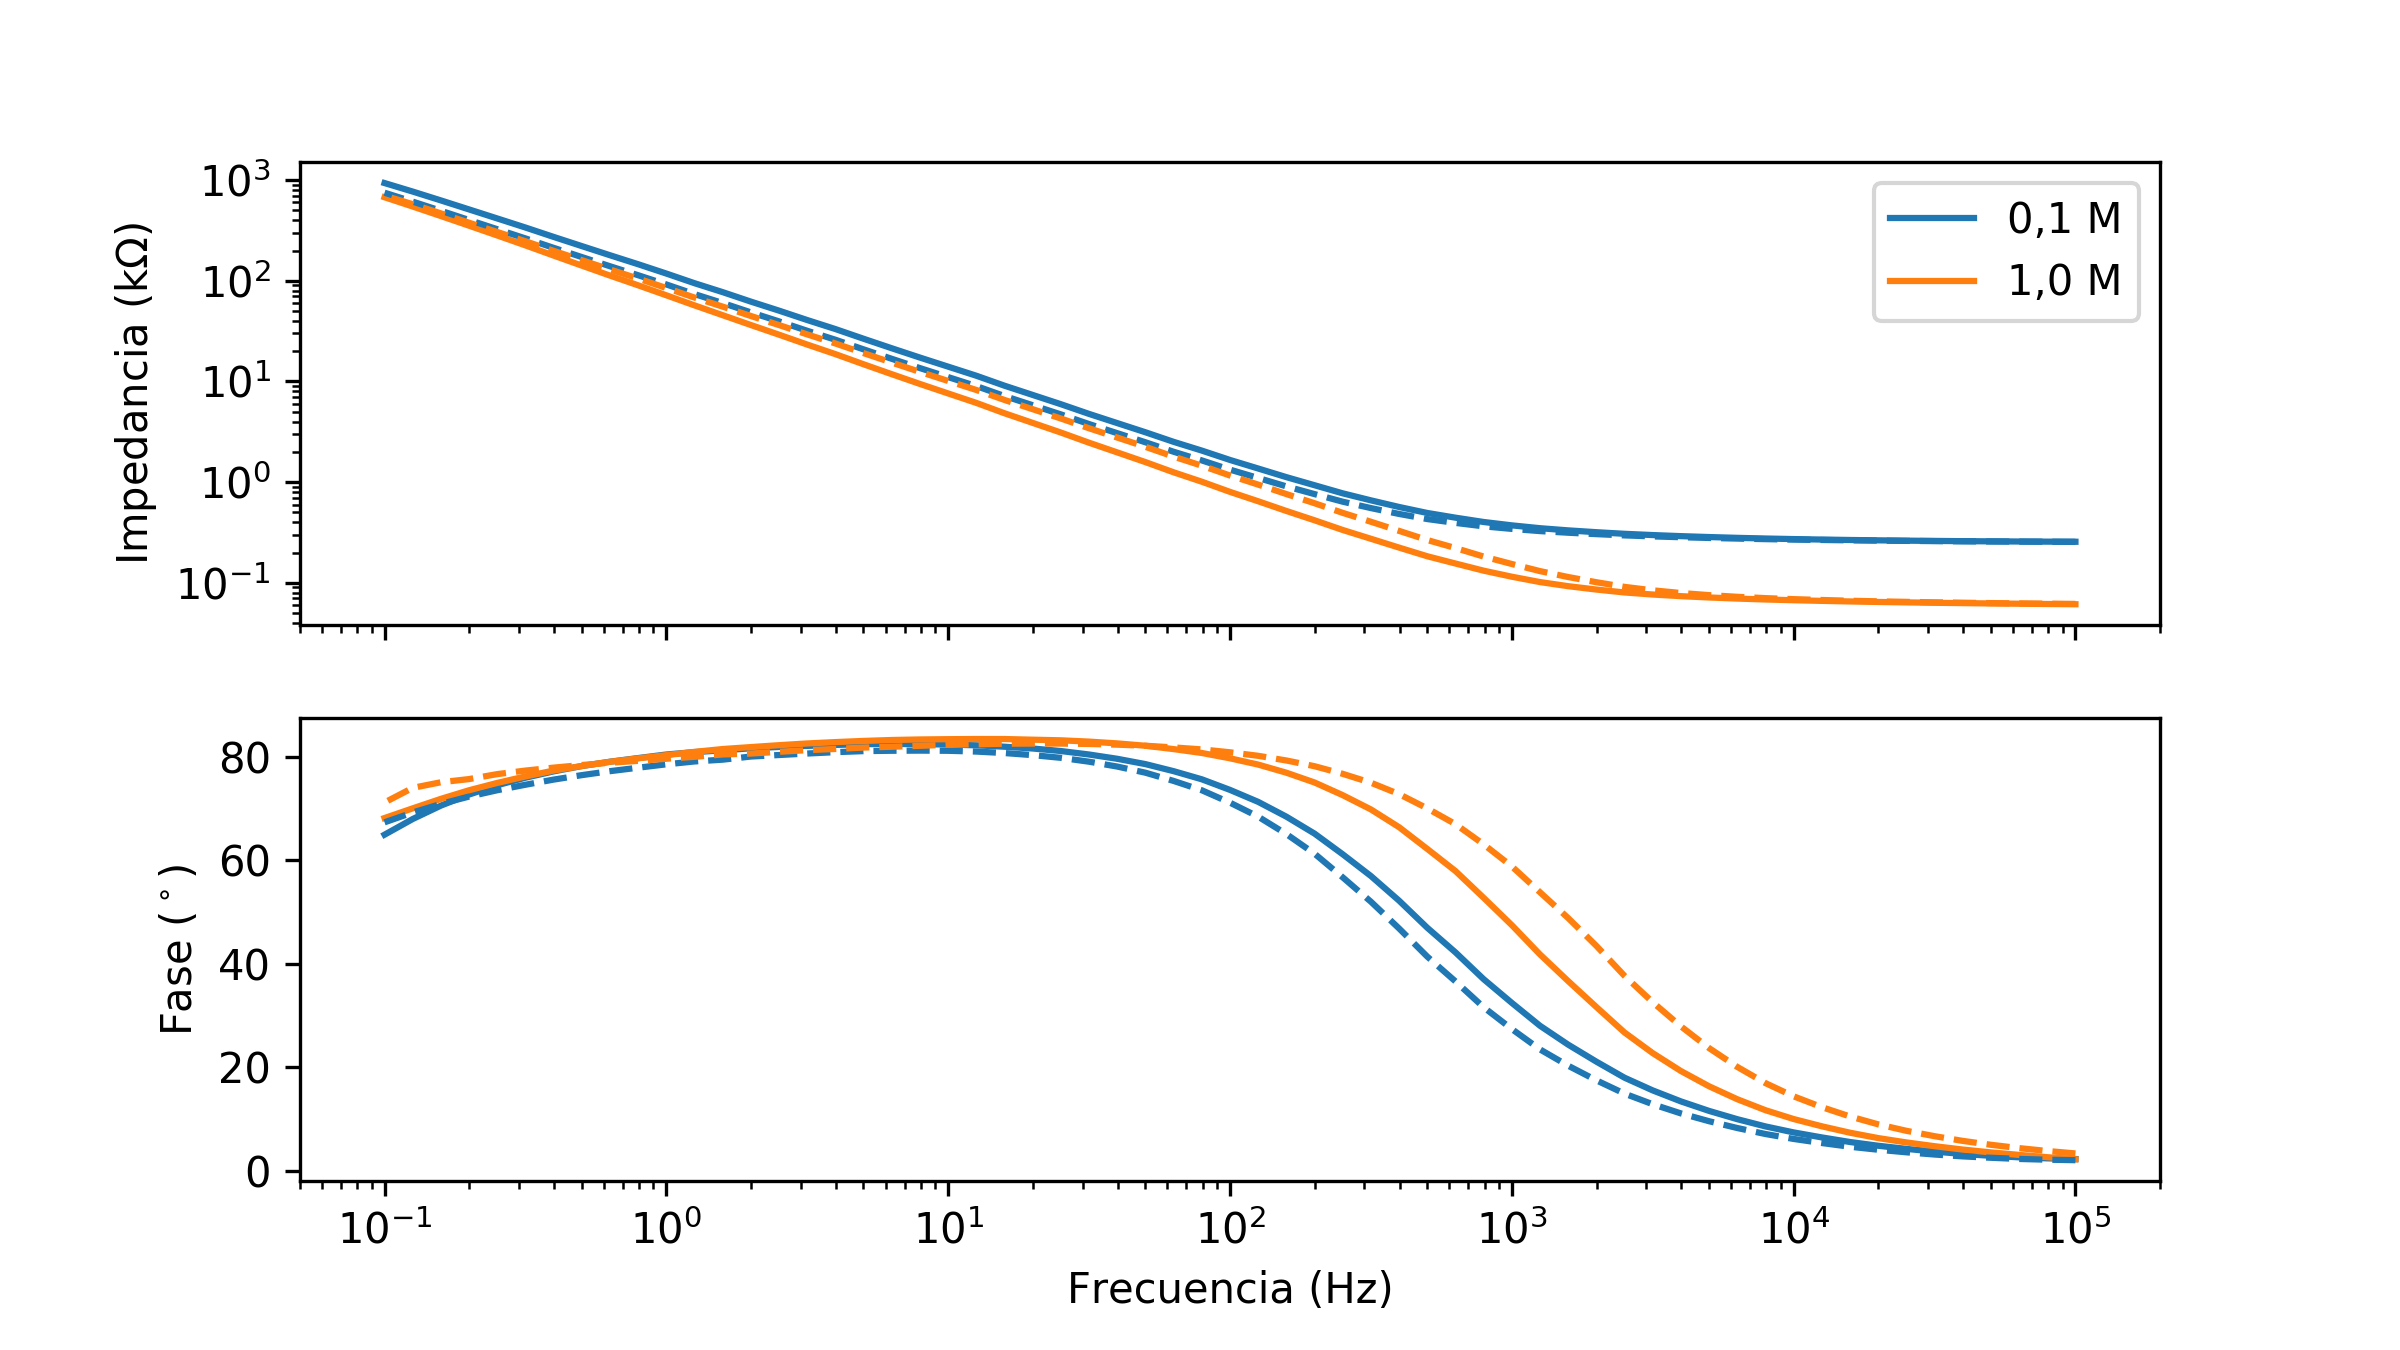
\includegraphics[width = \linewidth]{LiClO4_voltages}
		\caption{Valores de impedancia en funci\'on de la frecuencia (superior) y diagrama de Bode (inferior) de la soluci\'on de \ce{LiClO4} a diferentes concentraciones. En lineas cont\'inuas 0,0 V y en segmentos 0,3 V.}
		\label{fig: voltajes}
	\end{figure}
	
	En la \autoref{fig: voltajes} se observa el cambio de la impedancia en soluciones de la misma concentración a diferente voltaje. Es evidente que el voltaje aplicado cambia la capacitancia como se observa al comparar los valores de CPE a la misma concentración, pero a diferente voltaje en la \autoref{tb: 0,0} y \autoref{tb: 0,3}. Esto es un aspecto que puede ser explicado con la teoría de Gouy-Chapman-Stern, con esto se considera que hay una variación en la capacitancia cuando hay una diferencia de voltaje con respecto al potencial Z. Este efecto es más notorio es sistemas de baja concentración del electrolito \cite{bard2001fundamentals}.
	
	\begin{figure}[h]
		\centering
		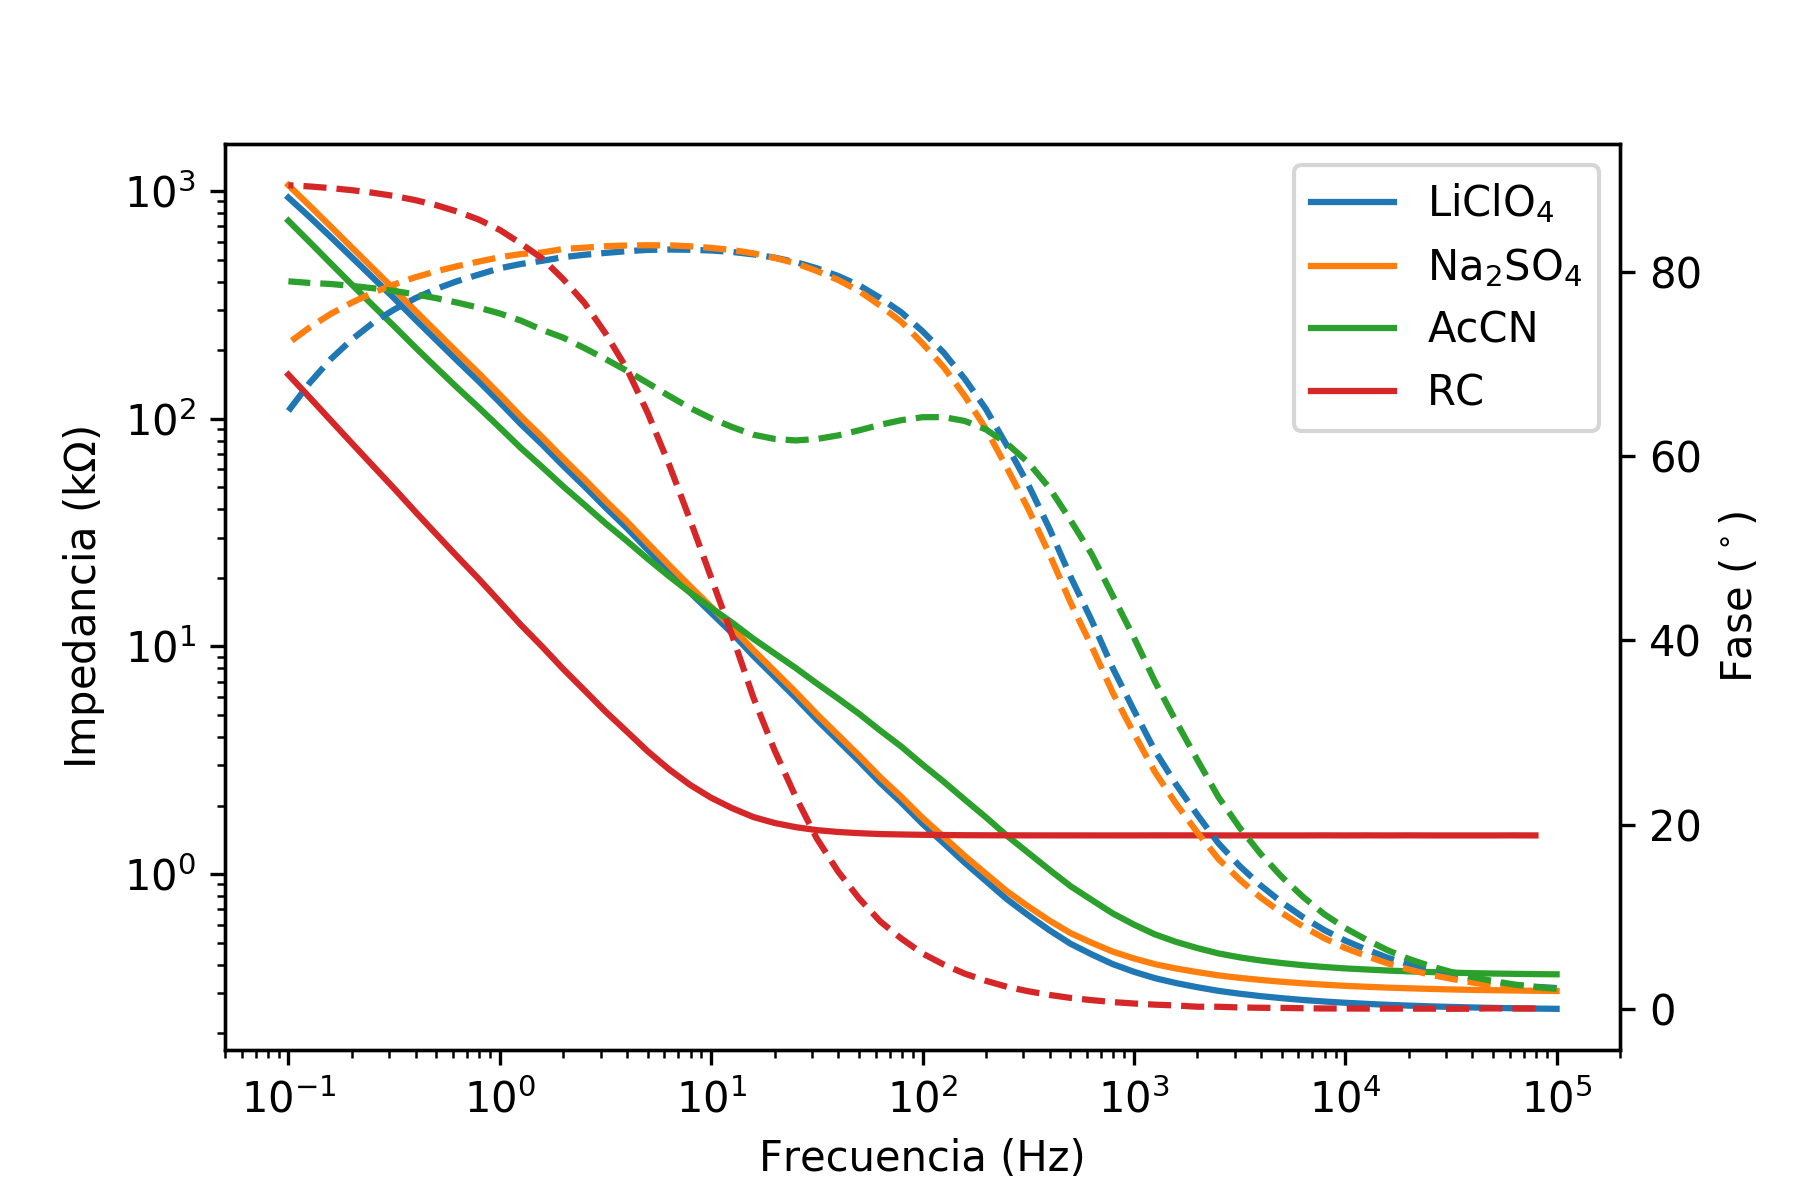
\includegraphics[width = \linewidth]{Iones}
		\caption{Impedancia de \ce{Na2SO4} 0,1 M en agua (naranja), \ce{LiClO4} 0,1 M en agua (azul) y 0,1 M en acetonitrilo (verde). En l\'ineas continuas se muestra la impedancia.}
		\label{fig: iones}
	\end{figure}
	
	En la \autoref{fig: iones} se observa que a 0,0 V no hay una diferencia en la impedancia entre el \ce{LiClO4} y el \ce{Na2SO4}, esto parece ser un efecto similar al que se observa en la \autoref{fig: concentraciones}, en la que el cambio de concentración no parece ser tan influyente en la impedancia a 0,0 V como si lo es a 0,3 V. También se observa que la solución de \ce{LiClO4} en acetonitrilo tiene un comportamiento muy distinto al del agua. Este efecto del solvente está dado porque la constante dieléctrica del acetonitrilo es menor, afectando su comportamiento electroquímico. 
	
	Como fue mencionado anteriormente es posible asociar un circuito ideal al efecto observado, dado que para los valores obtenidos de $n$ para las soluciones de \ce{LiClO4} a distintas concentraciones y potenciales es cercano a 1. De esta manera se tiene que para el capacitor en paralelo con la resistencia se tendr\'a una impedancia equivalente:
	\begin{equation*}
		Z_{eq} = \dfrac{Z_2Z_c}{Z_2 + Z_c} = \left(\dfrac{R_2}{j\omega C}\right)\dfrac{1}{(R_2 + 1/(j\omega C))}
	\end{equation*}
	\begin{equation}
		Z_{eq} = \dfrac{R_2}{j\omega R_2C + 1} = \dfrac{R_2 - j\omega CR_2^2}{1+(\omega R_2C)^2}
	\end{equation}
	
	Donde $\omega$ corresponde con la frecuencia angular, esto es: $\omega = 2\pi f$, con $f$ la frecuencia en Hz. Considerando ahora la resistencia de la soluci\'on, se tiene que la impedancia total $Z$ est\'a dada por la siguiente ecuaci\'on:
	\begin{equation}
		Z(\omega) = R_1 + Z_{eq} =  R_1 + \dfrac{R_2 - j\omega CR_2^2}{1+(\omega R_2C)^2}
	\end{equation}
	En particular se tiene que para $\omega \rightarrow 0$, $Z = R_1 + R_2$ y para $\omega \rightarrow \infty$ se tendr\'a $Z = R_1$. Lo cual explica la alta impedancia observada a bajas frecuencias, y su estabilizaci\'on a altas. Para la fase se tiene:
	
	\footnotesize
	\begin{equation}
		\theta = \arctan\left(\dfrac{Im(Z)}{Re(Z)}\right) = \arctan\left(\dfrac{R_2^2C\omega}{R_1(R_2C\omega)^2 + R_1 + R_2}\right)
	\end{equation}
	\normalsize
	
	Para lo cual en ambos l\'imites $\omega\rightarrow 0$ y $\omega\rightarrow \infty$, se tiene $\theta = 0$. Esto explica c\'omo cae la fase para valores altos de frecuencia, y el incremento de la misma a valores bajos. M\'as a\'un, la derivada del mismo determina la posici\'on del punto cr\'itico.
	
	\footnotesize
	\begin{equation}
		\left(\dfrac{d\theta}{d\omega}\right)_{\omega_0} =  \dfrac{CR_2^2\left(R_1 + R_2 -R_1(R_2C\omega_0)^2\right)}{R_2^4C^2\omega_0^2 + \left(R_1 + R_2 + R_1(R_2C\omega_0)^2\right)^2} = 0
	\end{equation}
	\normalsize
	
	De donde se obtiene que el m\'aximo de fase estar\'a dado por:
	\begin{equation}
		\omega_0 = \dfrac{\sqrt{R_1 + R_2}}{C\sqrt{R_1R_2}}
	\end{equation}
	
	De acuerdo con los valores de la \autoref{tb: 0,0} y \autoref{tb: 0,3} las frecuencias corresponden a: 3.65 Hz y 6.97 Hz, 2.95 Hz y 5.78 Hz correspondientemente para las concentraciones de 0,1 M y 1,0 M a 0,0 V y 0,3 V. Lo anterior constituye una prueba adicional de los valores de $n$ mostrados en las mismas tablas, pues las frecuencias son cercanas a las observadas en la \autoref{fig: concentraciones}.
	
	Ahora, en particular para el circuito ideal RC, se tiene una resistencia $R$ en serie con un capacitor $C$, de tal forma que la impedancia est\'a dada por:
	\begin{equation}
		Z(\omega) = R + \dfrac{1}{j\omega C} = R - \dfrac{j}{\omega C}
	\end{equation}
	
	De tal forma que a frecuencias bajas la impedancia es grande dada la divergencia de $\omega$, y a frecuencias altas tiende a $R$, comportamiento observado en la \autoref{fig: iones}. La fase est\'a dada por:
	\begin{equation}
		\theta = \arctan\left(\dfrac{1}{RC\omega}\right)
	\end{equation}
	
	Dada la forma asint\'otica de la funci\'on arcotangente, para $\omega\rightarrow0$ la funci\'on est\'a definida y tiende a 90 $^\circ$, y en $\omega\rightarrow\infty$ tendr\'a valor cero. Dicho comportamiento tambi\'en se evidencia en la \autoref{fig: iones}. A partir de este an\'alisis es posible concluir que tanto el sistema ideal como el sistema electrolito/electrodo tienen comportamientos an\'alogos pues la forma de las curvas es la misma.
	
	\section{Conclusiones}
	
	
	%----------------------------------------------------------------------------------------
	%	REFERENCE LIST
	%----------------------------------------------------------------------------------------
	\phantomsection
	\bibliography{informe}
	\bibliographystyle{achemso}
	
	
\end{document}